\chapter{Support Vector Machines}
\section{Theory}

In this section of the appendix the soft margin support vector machine (SVM) is described. The SVM is a binary classifier, which is a problem with multi class. 
The solution for multiclass classification is using a one-vs.-one setup.
With only three classes this is achieved with relative ease. 
The integrated MATLAB statistic toolbox was used to process the data in the SVM case. 

SVM classify by making a decision boundary that maximizes the margin $ \gamma $.
The margin is the perpendicular distance from the decision boundary to the closest feature point.
The standard SVM have a linear decision boundary, which classifies by assigning the new data point to either class $ t=1 $ or $ t=-1 $. 
The decision function for a standard SVM for a test point $ x_{new} $ given by
\begin{equation}
t_{new} = \mathtt{sign}(\mathbf{w}^T \mathbf{x}_{new} +b)
\label{eq:SVM_lin}
\end{equation}
The parameter vector $ \mathbf{w} $ is found by maximizing the margin or minimizing the length of the parameter vector, because of the inverse relationship $ \gamma = \frac{1}{\|\mathbf{w}\|} $.
Moving one single data point can have a huge influence on the position of the decision boundary, The reason is in the constrain
\begin{equation}
\qquad \mathbf{w}^* =
\mathtt{argmin}_\mathbf{w} \frac{1}{2} \mathbf{w}^T \mathbf{w}, 
\qquad t_n(\mathbf{w}^T \mathbf{x}_n + b) \geq 1
\end{equation}   
This however means that all the training features have sit on the correct side of the decision boundary.
This way of classifying is called hard margin SVM, which can't handle overlapping classes.
Therefore a slacken of the constrains is introduced $ \xi_n \geq 0 $ along with a regularization parameter \textit{C}, This is called soft margin SVM
\begin{equation}
\mathbf{w}^* = 
\mathtt{argmin}_\mathbf{w} \frac{1}{2} \mathbf{w}^T \mathbf{w}+C \sum_{n=1}^{N} \xi_n, \qquad t_n(\mathbf{w}^T \mathbf{x}_n + b) \geq 1-\xi_n
\end{equation} 
This optimization problem can be rewritten into the following quadratic problem by using Lagrange multipliers
\begin{equation}
\alpha^* = 
\mathtt{argmin}_\alpha \sum_{n=1}^{N}\alpha - \frac{1}{2} 
\sum_{n,m-1}^{N} \alpha_n \alpha_m t_n t_m \mathbf{x}^T_n \mathbf{x}_m, 
\qquad \sum_{n=1}^{N} \alpha_n t_n = 0, \qquad
0\leq \alpha_n \leq C 
\end{equation}
The influence of each training point in the decision boundary is proportional to $ \alpha_n $.
After the training process, the classification can be done by using the following expression, where $ \mathbf{x}_n $  are the support-vectors, and $ \alpha_n $ is their weights.
\begin{equation}
t_{new} = 
\mathtt{sign}(\mathbf{w}^T \mathbf{x}_{new} +b) =
\mathtt{sign}\left( \sum_{n=1}^{N} \alpha_n t_n \mathbf{x}^T_n \mathbf{x}_{new} +b  \right) 
\end{equation} 
Instead of using a linear decision boundary, different kernels can be used to make other decision boundary.
There are a linear kernel $ \mathbf{x}^T_n \mathbf{x}_{new} $, polynomial kernel $ (\gamma \mathbf{x}^T_n \mathbf{x}_{new} )^d,\; \gamma > 0 $.
The kernel used in this project is the radial basis function $ \mathtt{exp}(-\gamma \|\mathbf{x}^T_n - \mathbf{x}_{new} \|^2 ), \; \gamma > 0 $, also called the Gaussian kernel.

To expand this binary classifier to being able to process multiclass classification a one-vs.-one setup is used. 
This means that each of the classes is trained against all of the other classes, this results in $ k(k-1)/2 $ classifiers. 
The class assignment is then based on a voting between the different classifiers. 
This is implemented by evaluating the classifier between the $ i^{th} $ and the $ j^{th} $ class.
If the classifier says $ \mathbf{x}_{new} $ is in the $ i^{th} $ class this class is raised with one.
The class which has received the most votes is then the winning class.
 
\section{Method}
the implementation of the SVM classifier, the soft margin version was used.
The kernel used in this project was the Gaussian kernel.  
The three classes in this case is determined by the one-vs.-one setup. 
250000 iterations took

\section{Results}

\begin{figure}[H]
\centering
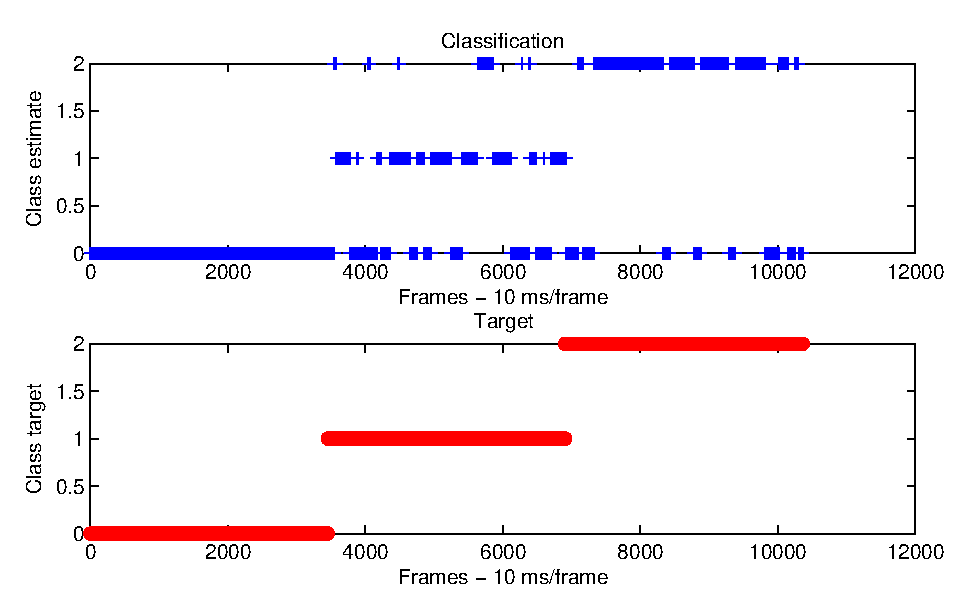
\includegraphics{SVM_3_1digit_PCA10}
\caption{Results of using SVM classifiers and one digit spoken}
\label{fig:SVM3_1dig_PCA}
\end{figure}

\begin{table}[H]                                                    
\centering                                                          
\begin{tabular}{|l|c|c|c|c|}                                        
\hline                                                              
  & Speaker Jacob & Speaker Mose & Speaker Simon & Precision [\%] \\
\hline                                                              
Estimate Jacob & 3454.0 & 1408.0 & 1002.0 & 58.9 \\                 
\hline                                                              
Estimate Mose & 0.0 & 1746.0 & 12.0 & 99.3 \\                       
\hline                                                              
Estimate Simon & 0.0 & 300.0 & 2440.0 & 89.1 \\                     
\hline                                                              
Sensitivity [\%] & 100.0 & 50.6 & 70.6 & 73.7 \\                    
\hline                                                              
\end{tabular}                                                       
\caption{Confusion matrix - 1 digit}                                
\label{table:SVM_3_conf_1}                                          
\end{table} 


\section{Discussion}
The SVM was applied on the dataset containing tree speakers saying one digit.
The model was not applied on the other dataset because the large number of iteration it took to get a result.
The other reason is that the result of the smallest data isn't the best 
The confusion matrix is shown on table \ref{table:SVM_3_conf_1} and having a overall accuracy of 73,3 \%.